\chapter{Modèle Solid-On-Solid}

La discrétisation du champ $\phi(\mx,t)$ afin de faire des simulations numériques mène naturellement vers le modèle sur réseau par excellence, le modèle d'Ising. À partir de deux dimensions, ce modèle de particules à interaction avec les plus proches voisins possède une transition de second ordre depuis une phase ordonnée vers une phase désordonnée, dont - si on suppose l'énergie d'interaction entre toutes les particules plus proches voisins égale à $J$ - la température critique est $\beta_{C,2D} =  \frac{\ln(1+\sqrt{2})}{2} J \simeq 0.44 J$ en deux dimensions \cite{onsager_crystal_1944} et $\beta_{C,3D} \simeq 0.22 J$ en trois dimensions \cite{talapov_magnetization_1996} (via des simulations de Monte Carlo).

À basse température $T \less T_C$, le système tend à créer des domaines de magnétisation moyenne opposées induisant des interfaces. Nous rappelons dans ce chapitres quelques notions essentielles sur le modèle d'Ising, sur la manière d'étudier les interfaces dans ce modèles, et une approximation à très basse température qui ne retient que l'information sur l'interface : le modèle Solid-On-Solid.

		  \section{Le modèle d'Ising}
  
\begin{figure}
	\begin{minipage}[t]{0.5\linewidth}
		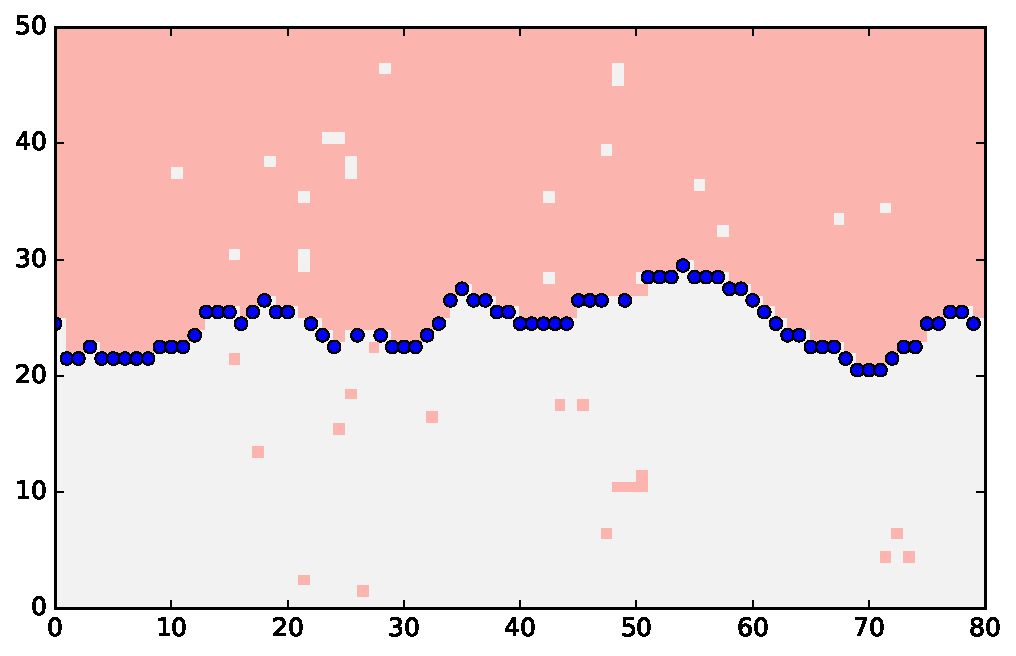
\includegraphics[width=\linewidth]{isingtosos/snap07.pdf}
	\end{minipage}%
	\begin{minipage}[t]{0.5\linewidth}
		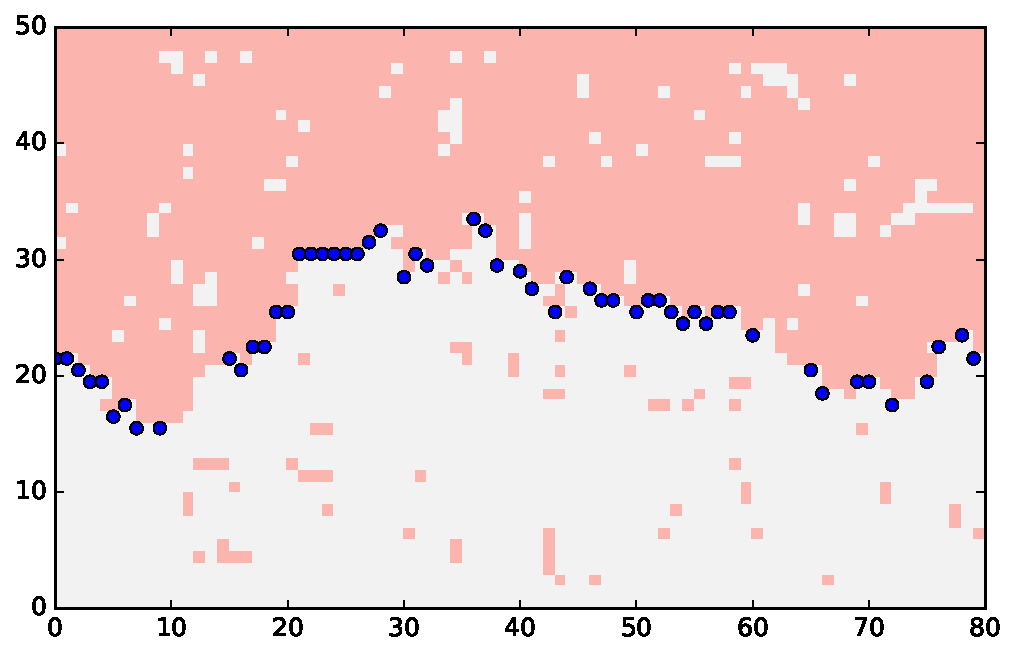
\includegraphics[width=\linewidth]{isingtosos/snap09.pdf}
	\end{minipage}
	\caption{Photo d'un modèle d'Ising à deux températures différentes($T=0.7 T_C$ et $T=0.95 T_C$ ) avec des conditions périodiques aux bords en X et fixés en Y qui forcent la présence d'une interface entre les phases $+$ (rose) et $-$ (blanc) du système. Plus la température est élevée et plus l'interface fluctue, jusqu'à cesser d'exister pour $T \greater T_C$. }
	\label{amas-fixe}
\end{figure}  
  
  	Le modèle d'Ising \footnote{Pour le lecteur curieux quant à l'histoire du modèle, se référer à \cite{niss_history_2005} et à \cite{niss_history_2009}.} est un modèle de particules sur réseau où l'interaction entre les particules du système se fait uniquement entre les plus proches voisins. Chaque particule au site $i$ possède deux états différents que l'on note $\sigma_i = \pm 1$, analogues aux spins en mécanique quantique. L'Hamiltonien d'un tel modèle s'écrit alors
\begin{equation}
	\mH =  - \sum_{<i j >} J_{ij} \sigma_i \sigma_j + \frac{V(i)+V(j)}{2}
\end{equation}
où $< ij >$ dénotent deux premiers voisins, $J_{ij}$ l'énergie d'interaction entre deux sites et $V(i)$ un champ externe. On peut voir ce terme d'interaction comme la discrétisation du terme $(\nabla \phi(\mx,t))^2$ où l'on a enlevé les constantes d'énergies, et l'absence du potentiel $\phi^4$ puisqu'il est toujours égal à $m^2+\frac{\lambda}{4!}$ ici. 

En faisant la transformation\cite{goldenfeld_lectures_2018} $n_i =  \frac{\sigma_i +1}{2}$ afin que $n_i(\sigma_i = 1) = 1$ et $n_i(\sigma_i = -1) = 0$, on obtient l'Hamiltonien
\begin{equation}
	\mH =  - \sum_{\langle i j >}  J_{ij} \left( 4 n_i n_j -2 ( n_i+n_j) + 1 \right)+ \sum_{\langle i j >}  J_{ij} \frac{V(\sigma_i)+V(\sigma_j)}{2}  
\end{equation}
où le terme constant $\sum_{\langle i j >}  J_{ij}$ ne modifie la fonction de partition $\mZ$ que d'une constante. On définit alors 
\begin{equation}
	\mH_{LG} =  - 4 \sum_{\langle i j >}  J_{ij}  n_i n_j  + 2 \sum_{\langle i j >}  J_{ij}  (n_i+n_j) + \sum_{\langle i j >}  J_{ij} \frac{V(\sigma_i)+V(\sigma_j)}{2}  
\end{equation}
Le deuxième terme s'identifie à la présence d'un potentiel chimique pour les particules liquide-gaz. Une phase magnétique positive dans le modèle d'Ising s'apparente dès lors à un état de haute densité (un liquide), tandis qu'une phase négative est considérée comme une phase de basse densité, c'est-à-dire un gaz.
Ce modèle représente également un mélange binaire entre deux types de particules $A$ et $B$ comme par exemple un polymère dans un solvant, les particules identiques s'attirant tandis que les particules d'un type différent se repoussent. 

L'étude de l'interface entre les phases $+$ et $-$ nécessite la brisure de la symétrie de translation au sein du système. Cela peut se faire par des conditions aux bords non-périodiques dans une direction.
Dans ce cas on a par exemple les spins de la rangée $0$ étant positifs et ceux de la rangée $L_Y$ négatifs, des clusters vont se former et créer une interface au milieu. Il est possible de favoriser une phase par rapport à l'autre grâce à un potentiel chimique (ou champ magnétique) $V(h_i) = -h \sigma_i$. 
La création d'une interface peut également se faire par un champ externe assymétrique favorisant une phase au-dessus et l'autre en-dessous, comme le potentiel $V(y) = - B |\frac{L_Y}{2}-y|$. Cette séparation modélise quant à lui l'effet d'un champ  sur un liquide binaire comme dans les expériences de forçage laser \cite{girot_conical_2019}. 

La tension superficielle d'une telle interface est alors donnée \cite{abraham_transfer_1973,abraham_interface_1976} par
\begin{align}
    \sigma = 2 \beta J - \log(\tanh(\beta J))
\end{align}
En absence de champ externe, 

L'épinglage\cite{} (\textit{pinning}) de l'interface auprès de la ligne de démarcation permet de l'étudier loin des bords du système.		
		
		\section{Hamiltonien}
	
Quelle que soit la méthode utilisée, le système se simplifie dès lors que nous désirons étudier uniquement l'interface d'un système et non son ensemble, telles que les longueurs de corrélations dans le \textit{bulk}, l'aimantation moyenne, la chaleur spécifique ou la susceptilibté magnétique. À très basse température, les interfaces sont bien délimitées et il y a très peu de gouttes d'évaporations d'une phase dans l'autre. En considérant le système très peu mélangé, il est possible de définir la présence d'une phase par rapport à la hauteur $h_i$ de l'interface. Chaque site prend la valeur
\begin{align*}
	\sigma_{i,j} = \sgn(h_i-j)
\end{align*}
où la fonction $\sgn(x)$ est égale à $+1$ si $x>=0$ et à $-1$ sinon. Cela revient à considérer que l'énergie d'interaction perpendiculaire est prohibitif par rapport aux liaisons parallèles à l'interface $J_\perp \gg J_\parallel$. 

\begin{figure}
	\centering
	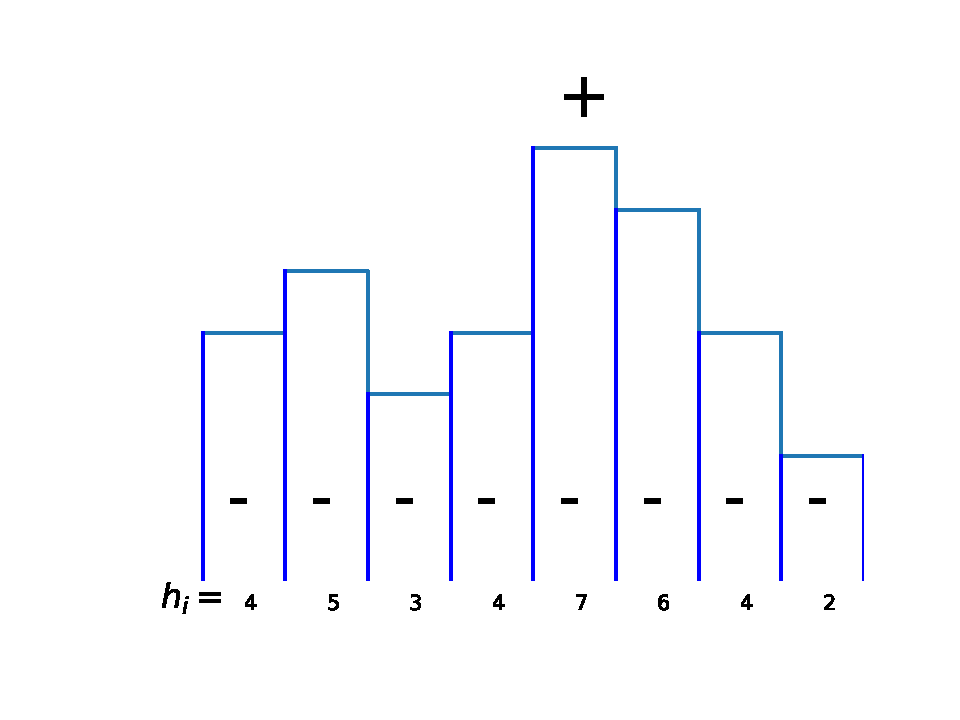
\includegraphics[scale=1]{isingtosos/sos-indiscernable.pdf}
	\caption{Une configuration possible de modèle SOS. Dans la i-ème colonne le bord horizontal de l'interface passe à la hauteur $h_i$. Toutes les particules au-dessus de l'interface sont des spins positifs et négatifs en dessous. La représentation classique du modèle SOS diffère de ce schéma par l'hypothèse que les particules sont discernables. Nous y reviendrons plus tard.}
\end{figure}


En utilisant l'identité $\min(a,b)-\max(a,b)=|a-b|$, on a
\begin{align*}
    \sum_{j=0}^L \sgn(h-j)\sgn(h'-j) = L - 2 |h-h'|
\end{align*}
Ainsi, pour un système de longueur $L_X$ et de largeur $L_Y$ l'hamiltonien du modèle d'Ising en absence de potentiel se réécrit comme 
\begin{align}
    \mH = 4 J L_X (2-L_Y) +4J \sum_i |h_i-h_{i+1}|
\end{align}
Le terme $|h_i-h_{i+1}|$ représente la surface de contact horizontale entre les deux phases qui dépend directement de la hauteur, tandis que le terme constant représente la surface de contact verticale.
En retirant la partie constante de l'énergie et simplifiant $4 J = J$ et en gardant $L_X = L$, nous obtenons l'hamiltonien du \textbf{modèle Solid-On-Solid}
\begin{align}
    \mH = J \sum_i |h_i-h_{i+1}|
    \label{hamil-sos}
\end{align}

Nous avons ici réussi à réduire la dimensionalité du système en ne prenant en compte que la hauteur $h_i$ au site $i$. L'énergie du système est alors décrite par la différence de hauteur entre deux sites voisins, et $\beta J$ prend ici alors le rôle de la tension de surface.

Puisqu'il n'y a plus de transition de phase possible dans ce modèle, la température critique $\beta_C$ du modèle d'Ising n'a plus de rôle à jouer ici. Pour rester dans le domaine de l'approximation, si nous désirons comparer les résultats avec ceux du modèle d'Ising, il faudra veiller à rester dans le domaine $T \less T_C$, l'approximation étant de plus en plus valable plus la température est basse. Par la suite, puisque nous désironts étudier le modèle SOS et non le comparer avec le modèle d'Ising, nous prendrons, sauf cas contraire explicité, $\beta = \beta_C \simeq 0.44$ et $J=1$ par soucis de simplicité. 

  \section{Matrice de Transfert}

	De manière plus générale, l'Hamiltonien d'un système avec des interactions entre les particules peut se réécrire comme $\mH = \sum_{\langle ij >} H(i,j)$ avec
\begin{align*}
  H(h_i,h_{i+1}) = f(h_i,h_{i+1}) + V(h_i,h_{i+1}) 
\end{align*}
où $f(h_i,h_j)$ est l'énergie d'interaction entre plus proches voisins et $V(h_i,h_j)=\frac{V(h_i)+V(h_j)}{2}$ le potentiel symmétrisé.
La fonction de partition de notre système s'écrit alors 

\begin{align*}
 Z = \sum_{h_1=0}^\infty \sum_{h_2=0}^\infty ... \sum_{h_L=0}^\infty e^{- \beta \sum_{i} H(h_i,h_{i+1})}  
   = \sum_{h_1 h_2 ... h_L} \prod_{i} e^{-\beta H(h_i,h_{i+1})} 
\end{align*}

\begin{figure}
    \begin{align}
    T = \begin{bmatrix} 
            \ddots & \vdots & \reflectbox{$\ddots$} \\ 
            e^{-\beta H(-1,-1)} &  e^{-\beta H(-1,0)} & e^{-\beta H(1,-1)} \\
            \dots & e^{-\beta H(0,0)} & \dots  \\
            e^{-\beta H(1,-1)} & e^{-\beta H(1,0)} & e^{-\beta H(1,1)}   \\ 
             \reflectbox{$\ddots$} & \vdots &\ddots  \\ 
        \end{bmatrix}
    \end{align}
    \caption{Matrice de transfert infinie et symmétrique \ref{matric-transfert}.}
\end{figure}

La matrice 
\begin{align}
    T(h_i,h_j) = e{-\beta H(h_i,h_j)}
    \label{matric-transfert}
\end{align}
est appelée matrice de transfert. Puisque le système est pérdioque (c'est-à-dire que $h_{L+1} = h_1$,  la matrice est périodique également, c'est-à-dire $T(h_L,h_{L+1}) = T(h_L,h_1)$. Elle est également symétrique, ce qui implique qu'elle est diagonalisable dans la base des vecteurs propres $|\lambda >$ de valeur propre $\lambda$. On dénote par $\lambda_0$ la plus grande valeur propre de $T$, par $\lambda_1$ la deuxième plus grande valeur propre et ainsi de suite.
Ainsi on peut diagonaliser la fonction de partition par la trace de la matrice de transfert
\begin{align}
  Z = \sum_{h_1 h_2 ... h_L} \prod_{i} T(h_i,h_{i+i}) = Tr T^L  = \sum_\lambda \langle\lambda | T^L | \lambda> = \sum_\lambda \lambda^L
\end{align}

Dans la limite thermodynamique $L \to \infty$, seuls les plus grands vecteurs propres jouent un rôle. Afin de calculer les observables de notre système, il convient d'introduire les vecteurs de l'espace de Hilbert de ${|\lambda>}$ qui vont de $|h = -\infty>$ à $|h = +\infty>$.
En introduisant également la matrice des hauteurs $\tilde{M} |h> = h |h> i$, on trouve
\begin{itemize}
	\item L'énergie libre par site :  
	\begin{align}
		F =  - \frac{1}{L \beta} \ln(Z) \simeq - \frac{1}{L \beta } \ln( \lambda_0)
	\end{align}
	\item La densité de probabilité qu'un site se trouve à la hauteur $h$ avec
	\begin{align}
		p(h) = \frac{1}{Z} \sum_\lambda \lambda^L \langle\lambda | h >^2 \simeq \langle \lambda_0 | h >^2
	\end{align}
	\item La magnétisation moyenne :
	\begin{align}
		M = \langle h > = \langle \lambda_0 | \tilde{M} | \lambda_0 > 
	\end{align}
	\item La variance des hauteurs :
	\begin{align}
		\sigma = \langle (h - \langle h >)^2 > =  \langle \lambda_0 | \tilde{M}^2 | \lambda_0 >
	\end{align}
\end{itemize}

	\section{Stabilité de l'interface}

	Soit $\psi_\lambda(h)= <h|\lambda>$ la projection du vecteur propre associé à la valeur propre $\lambda$ de la matrice de transfert sur la base des hauteurs $|h>$ dans un système infini de par et d'autre de l'interface. En absence de potentiel\cite{guyer_sine-gordon_1979}, l'équation du vecteur propre donne
\begin{align}
	\sum_{h=-\infty}^\infty T(h,h') \psi_\lambda(h) = \lambda \psi_\lambda(h')
\end{align}
En introduisant l'ansatz $\psi_\lambda(h) = \alpha_{\lambda}^h$ qui respecte la symétrie du système, et en séparant de la somme les termes pour $h$ négatifs et positifs, on trouve aisément que 
\begin{align}
	\frac{\sinh(\beta J)}{\cosh(\beta J)-(\alpha_{\lambda}+\frac{1}{\alpha_{\lambda}})} = \lambda
\end{align}
Dans la limite thermodynamique, la probabilité de présence de l'interface à la hauteur $h$ est $p(h) = <\lambda_0|h>^2 = |\psi_0(h)|^2$. Le système ne possédant aucune brisure de symétrie particulière, la probabilité $p(h)$ se doit d'être bornée pour tout $h$. Dès lors, l'ansatz supposé $\psi_\lambda(h) = \alpha^h$ implique que $\alpha_{\lambda}$ soit de la forme $e^{ik}$ où $k$ est la longueur d'onde associée à la valeur propre $\lambda$. On obtient que 
\begin{align}
	\psi_k(h) =& e^{ikh} \\
	\lambda =& \frac{\sinh(\beta J)}{\cosh(\beta J) - \cos(k)}
\end{align}


Dans le cas plus général où la matrice de transfert s'écrit de la forme $T(h,h') = f(|h-h'|)$, on trouve 
\begin{align}
	\lambda = \sum_{h=0}^\infty f(h)(\alpha_{\lambda}^h+\alpha_{\lambda}^{-h}) - f(0)
\end{align}

L'existence d'une solution de ce genre indique que l'interface n'est pas localisée dans le cas d'un système infini (ou semi-infini) en absence de tout potentiel, ce qui conduit à de nombreux problèmes numériques. 

Il est à noter qu'à $\beta=0$, c'est-à-dire pour une température infinie, tous les termes de la matrice de transfert sont égaux à $1$, menant à des vecteurs propres nuls. Dans cette limite, l'interface n'existe plus, le modèle SOS n'est donc pas valable. De même, pour une température nulle $\beta=\infty$, la matrice de transfert devient la matrice identité. Les valeurs propres deviennent toutes égales à $1$ et les vecteurs propres sont $\psi_i(h) = \delta_{h,i}$ où ici $i$ est l'indice de la i-ème valeur propre $\lambda_i = 1$. La probabilité de trouver l'interface à la hauteur $h$ devient $p(h) = \frac{1}{Z}\sum_{i} <\lambda_i | h >^2 = 1$. La température nulle a pour effet de geler l'interface sur une seule hauteur, mais toutes les hauteurs sont équiprobables. Bien que les micro-états soient extrêmement différents que pour une température finie, les propriétés macroscopiques sont identiques à cause du même poids statistique associé à chaque état.


Historiquement, une manière facile de localiser l'interface est de rajouter un potentiel $V(h) = -B \delta_{h,0}$ \cite{chui_pinning_1999}. La présence du potentiel n'affecte pas la parité du système mais peut introduire un surplus de particules en $0$. La recherche d'un état localisé nous donne un ansatz de la forme 
\begin{align}
	\psi_\lambda(h) = \begin{cases} |\alpha|^h & \text{si } h \neq 0 \\ \psi_{\lambda,0} & \text{sinon} \end{cases} 
\end{align}
L'équation du vecteur propre devient
\begin{align}
	\sum_{h=-\infty}^\infty e^{\beta |h-h'|- \beta B \delta_{h,0}} \psi_\lambda(h) = \lambda \psi_\lambda(h')
\end{align}
En notant $T(h,h') = R^{|h-h'|}$ pour $h \neq h' \neq 0$,  on obtient la même équation à un signe près dans l'exposant que l'on soit à $h'>0$ ou $h'>0$
\begin{align}
	\left( \frac{R}{\alpha} \right)^{\pm h'} \left[ \psi_{\lambda,0} + \frac{R \alpha}{1 - R \alpha} + \frac{\alpha}{R - \alpha} \right] + \left[ \frac{1}{1-R \alpha} - \frac{R}{R-\alpha} \right] = \lambda
\end{align}
Puisque cette équation est vraie pour tout $h'$, le premier terme doit être nul, ce qui nous donne
\begin{align}
	\psi_{\lambda,0} &= - \frac{\alpha}{R-\alpha}-\frac{R \alpha}{1-R \alpha} \\
	\lambda &= \frac{1}{1-R \alpha} - \frac{R}{R-\alpha}
\end{align}
L'équation du vecteur propre à $h'=0$ nous donne par ailleurs 
\begin{align}
	\psi_{\lambda,0} + 2 \frac{R \alpha}{1-R \alpha} = \lambda \psi_{\lambda,0} e^{-\beta B}
\end{align}
L'existence d'une solution cohérente $\alpha < 1$ autorise la présence d'une interface localisée grâce au pinning.

D'autres méthodes existent pour confiner l'interface. Le cisaillement d'une interface diminue sa largeur et permet de la localiser dans l'espace. On peut également proposer deux potentiels chimiques différents pour chaque phase à une hauteur de l'interface prédéfinie, comme le ferait un laser dans les expériences de cisaillement\cite{delville} dans un système semi-infini. Cet cas sera étudié plus loin. Dans un système infini, une autre possibilité est de définir un champ magnétique symétrique rendant plus difficile la présence de l'interface loin de $0$. Nous utiliserons ici un potentiel du style
\begin{align}
		  V(h) = B |h|
\end{align}

Il est facile de se convaincre que loin de $h=0$ le coût énergétique est si grand que la probabilité que l'interface s'y trouve soit petite, impliquant que l'interface est localisée. La position moyenne de l'interface se situe au minimum du potentiel qui est dans ce cas $0$. 


	\section{Ensemble canonique}

\begin{figure}[h]
	\centering
	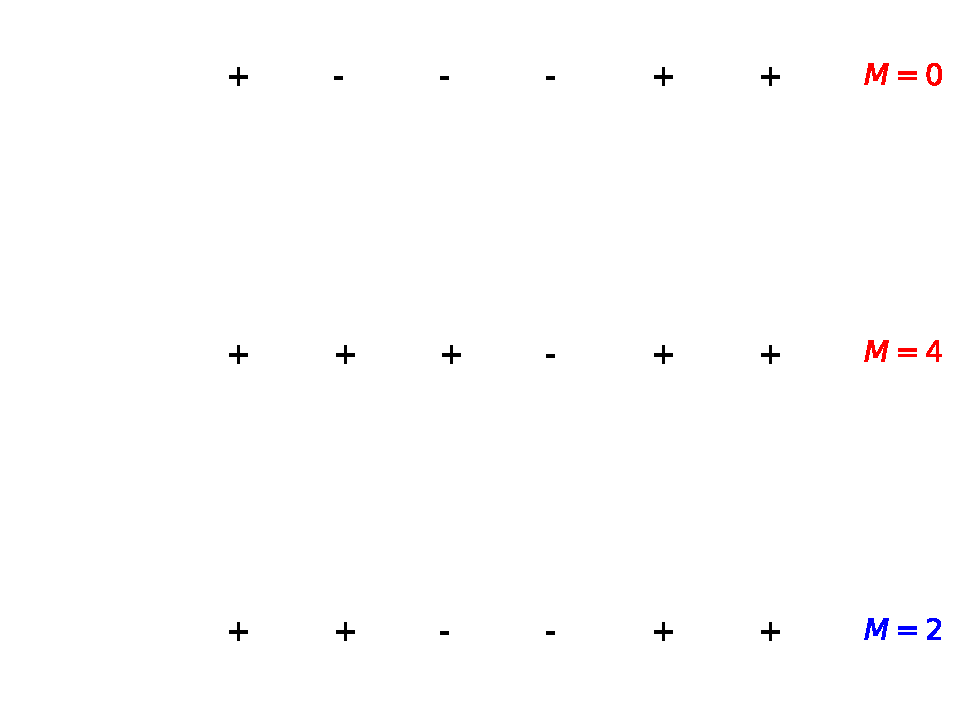
\includegraphics[scale=1]{isingtosos/figure-canonique.pdf}
	\caption{Dans un modèle d'Ising à 1D, afin d'avoir une magnétisation moyenne du système à $<M>=2$, tous les états sont acceptés tant qu'il y en a d'autres afin de respecter la moyenne. Dans l'ensemble canonique, on n'a plus $<M>=2$ mais $M=2$, interdisant les micro-états rouges.}
\end{figure}

Dans l'ensemble grand-canonique, le nombre de particules dans le système varie, dépendant du potentiel chimique vis-à-vis du réservoir dans lequel il est inséré, ce qui permet à l'interface de bouger librement. Lorsque l'on se place dans un système canonique, l'aire totale $A$ de l'interface soit fixe, ce qui introduit une contrainte dans la fonction de partition
\begin{align}
	 Z(A) = \sum_{h_1 h_2 ... h_L} e^{- \beta \sum_{i} H(h_i,h_{i+1})}  \delta(\sum_i h_i = A)
\end{align}
avec la relation vis-à-vis de l'ensemble grand-canonique pour un potentiel chimique $\mu$ donné
\begin{align}
	 \Xi(\mu) = \sum_{A = -\infty}^\infty Z(A) e^{\beta \mu M}
\end{align}
La position moyenne de l'interface est maintenant définie et beaucoup d'états sont interdits, ce qui change  les propriétés thermodynamiques de la matrice de transfert comme la distribution des hauteurs de l'interface, même si la moyenne reste la même. Dans la limite thermodynamique, si l'on prend dans l'ensemble canonique pour paramètre d'ordre la valeur moyenne du paramètre d'ordre dans l'ensemble grand canonique, on s'attend à ce que les observables du système se comportent de manière équivalente. 
Malheureusement, il est impossible de réécrire la contrainte dans le langage des matrices de transfert, empêchant ainsi de calculer analytiquement les différences entre les deux ensembles pour une taille donnée. Il est possible de construire la fonction de partition \textit{ab initio}, mais le grand nombre de sites et de hauteurs permises dans un système classique empêchent le calcul dans un temps CPU raisonnable. 


	\section{Indiscernabilité des particules : Particle-Over-Particle}
	
Dans le modèle d'Ising, les particules sont discernables puisque labellisées par leur position $(i,j)$. Cette discernabilité pose problème lorsque l'on utilise le modèle pour un système de gaz sur réseaux ou de fluides binaires par exemple. À cet égard le modèle SOS est meilleur, puisque la discernabilité ne concerne plus que les sites $i$ contenant $h_i$ particules indiscernables. 
En prenant le point de vue atomiste présent dans le modèle d'Ising, nous pouvons suivre la position de chaque particule au sein de nos sites. Cela a plusieurs implications.
La première, c'est qu'en général, seules les couches proche de l'interface sont actives, tandis que les mouvements dans le \textit{bulk} sont bien plus lents. Ainsi, en prenant une particule au hasard dans nos simulations numériques, il est possible de donner une mobilité différente aux couches du modèle SOS. Nous n'explorons pas ces systèmes dans la présente thèse. 
Deuxièmement, lors des algorithmes de Monte Carlo définit au chapitre suivant, la probabilité de choisir un site au hasard n'est pas la même que celle de choisir une particule au hasard ! 
La fonction de partition d'un système où les particules sont discernables s'écrit maintenant
\begin{align}
	Z = \sum_{h_1 h_2 ... h_L} e^{- \beta \sum_{i} H(i,i+1)} \frac{N!}{\prod_i n_i!} = N! \sum_{h_1 h_2 ... h_L} e^{- \beta \sum_{i} H(i,i+1) -\sum_i \ln(n_i!)}
\end{align}

Ce nouveau système, que l'on appellera - par analogie avec Solid-On-Solid - le modèle Particle-Over-Particle sera étudié de manière détailĺée dans les derniers chapitres.

\begin{figure}[h]
	\centering
	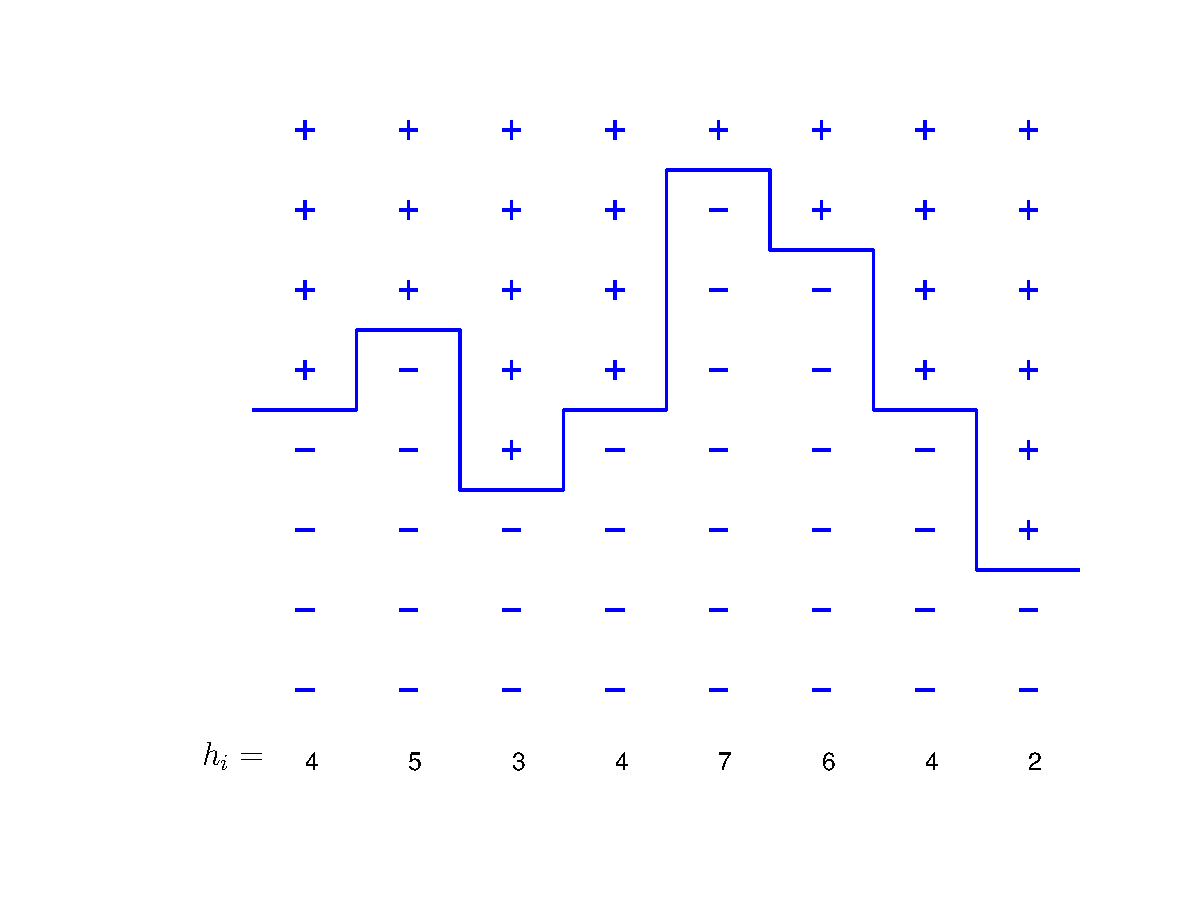
\includegraphics[width=0.7\linewidth]{isingtosos/figure-sos.pdf}
	\caption{Une configuration possible de modèle SOS lorsque les particules sont discernables. Cette représentation est la représentation classique dans la littérature.}
\end{figure}



\begin{comment}
		\section{SOS Hamiltonian}
		%%%%%%%%%%%%
		
		In the following, we present three Solid-On-Solid models with different magnetic fields. 
		The SOS interaction between nearest neighboors is of the form $f(i,j) = |h_i - h_j|$. 
		This kind of interaction prevents big fluctuations between two nearest neighboors and is directly related to the Ising model in the approximation where there are no overhangs between the two phases. \textcolor{blue}{see my notes for the derivation}
		
		In the absence of a magnetic field, the interface will fluctuate around its center. Shown below an typical SOS interface for an $L_X=50$ and a $L_Y=60$ after $10^5$ Monte Carlo steps.
		
		%\includegrapsics[width=10cm]{nomag.png}
		
		
		%%%%%%
		\subsection{Model $g(i) = h_i$ (model A)}
		%%%%%%
		
		This model replicates the effect of a homogeneous magnetic field. The bigger the magnetic field $B$ (which can be positive or negative), the further the interface is driven with a symetry breaking. 
		
		\begin{align}
		  H(i,j) = J |h_i-h_j| + B \frac{h_i + h_j}{2}
		\end{align}
		
		%\includegrapsics[width=10cm]{normal.png}
		
		For an infinite magnetic field, we clearly see that the interface gets flattened over on of the edge. The resulting single state avalaible in this limit is the flat interface, with all sites beeing over or under it, depending on the sign of $B$.
		
		In the limit $B \rightarrow \infty$, the interface will flatten to the bottom edge, resulting in a single state of energy 
		\begin{align}
		  F(B \rightarrow \infty) = - B L_Y
		\end{align}
		
		The free energy for at $B=0$ is thus given by align \ref{free_energy} as
		\begin{align}
		  F(0) = B L_X L_Y - \int_0^\infty m(B)dB
		  \label{energymodela}
		\end{align}
		with $m(B) = \langle\sum_i h_i> = L_Y$
		
		%%%%%%
		\subsection{Model $g(i) = |h_i|$ (model B)}
		%%%%%%
		
		This model uses a stagged magnetic field analoguous to the action of a laser on a binary mixture. The further we get from the mean position, the higher is the energy. In order to minimize the energy, the system will have a tendency to be pinned, leading to a very flat interface. 
		
		\begin{align}
		  H(i,j) = J |h_i-h_j| - B \frac{|h_i| + |h_j|}{2}
		\end{align}
		
		%\includegrapsics[width=10cm]{stagged.png}
		
		In the limit $B \rightarrow \infty$, the free energy $F$ will be equal to $0$, while the magnetisation $m(B \rightarrow \infty) = \langle\sum_i |h_i|> = 0$ also.
		
		%%%%%%
		\subsection{Model $g(i) = -|h_i|$ (model C)}
		%%%%%%
		
		This model is the same as the previous one, except with a switch of sign. In this case, the magnetic field will have a depinning effect leading to a scattering of the heights around both edges. \textcolor{red}{I don't really get yet the argument about the competition between entropy and energy.}
		
		\begin{align}
		  H(i,j) = J |h_i-h_j| - B \frac{|h_i| + |h_j|}{2}
		\end{align}
		
		%\includegrapsics[width=10cm]{negstagged.png}
		
		In the $B \rightarrow \infty$ limit, we have then a scattered system. How can we compute its free energy ? Sites will be at $h_i=\pm L_Y$ , leading to an easy $2\times 2$ transfer matrix.
		\begin{align}
		  Z = e^{\beta B L_Y L_X} Tr( (e^{-\beta J \frac{L_Y}{2} \sum_i |\sigma_i - \sigma_j| })^{L_X} )
		\end{align}
		where $\sigma_i = \pm 1$
		
		The transfer matrix is then given as
		
		\begin{align}
		T= e^{\beta B L_Y}
		  \begin{pmatrix}
		    1 & e^{-\beta 2 J L_Y} \\
		    e^{-\beta 2 J L_Y} & 1
		  \end{pmatrix}
		\end{align}
		Its eigenvalues are $\lambda_\pm = e^{\beta B L_Y}( 1 \pm e^{-\beta 2 J L_Y})$, giving a partion function 
		\begin{align}
		  Z = e^{\beta B L_Y L_X} \times ((1 - e^{-\beta 2 J L_Y})^{L_X} + (1 + e^{-\beta 2 J L_Y})^{L_X} )
		\end{align}
		
		The free energy from \ref{deffree_energy} is 
		\begin{align}
		  F(B\rightarrow \infty) = - L_Y B - \frac{1}{\beta} \ln \left( 1 + e^{-\beta 2 J L_Y} \right)
		  \label{energymodelc}
		\end{align}
		which, in the limit of $L_X \rightarrow \infty$ converges to \ref{energymodela}. This is easily explained as the energy to switch from a side to another increases so much that at some point the interface will be pinned to one of the edges, resulting in the same single state.
		
		\begin{figure}
		%  \includegrapsics[width=13cm]{comparison.pdf}
		  \caption{Computation of both terms in \ref{free_energy} in the limit $L_X \rightarrow \infty$ and $L_Y=30$ for the three different models. We see that models A and C have a very similar behaviour even for very small $B$. The linear fit does indeed give a relation $F(0) - F(B) = L_Y \times B$}
		\end{figure}
		
		%%%%%%%%%%%%
		\newpage
		\section{Numerical results}
		%%%%%%%%%%%%
		
		The diffusion of particles in a system can be mapped in an Ising model pretty easily if we assume the conservation of particles through time in our Monte Carlo dynamics. That means that $\sum h_i = K$, with $K$ a constant defined by the initial conditions. This condition can be enforced in the partition function if we only take the microstates satisfying our constraint. Sadly, this constraint is about the microstates and can not be transposed into our Hamiltonian, making the Transfer Matrix useless for such a case. 
		
		The question we want to adress is thus : how big is the difference between the constrained and the unconstrained dynamic in the computation of the free energy ? Is the limit $B^{\ast} \rightarrow \infty$ the same for the three models for both dynamics ? 
%		Figure \ref{compGlau} conforts us in the conformity between the Glauber dynamic and the Transfer Matrix method. 
		
		\begin{figure}[h]
		%  \includegrapsics[width=13cm]{ModGlau.pdf}
		  \caption{Computation of the free energy (above) and the magnetisation (below) for the three models in a Glauber dynamics (unconstrained dynamics) through simulations (with error bars) and exact transfer matrix diagonalization.}
		  \label{compGlau}
		\end{figure}
		
		When comparing to the Kawasaki dynamic in Figure \ref{compKaw}, we start seeing some differences. First, in model A the magnetization of our system is always  equal to $0$, by construction of our Kawasaki dynamics, meaning that the computation of the free energy is a tricky one. Luckily, Model A is very similar to Model C with respect to the posible microstates, except some walls that do not add a significan free energy into the system. This means that the results we obtain in Model C are roughly the same as in Model A ! This allows us to drop Model A from the discussion from now on and get retrieve its general behaviour and properties from Model C.
		
		As expected, the constrained dynamics adds some variance with respect to the Transfer Matrix. 
		
		\begin{figure}
		%  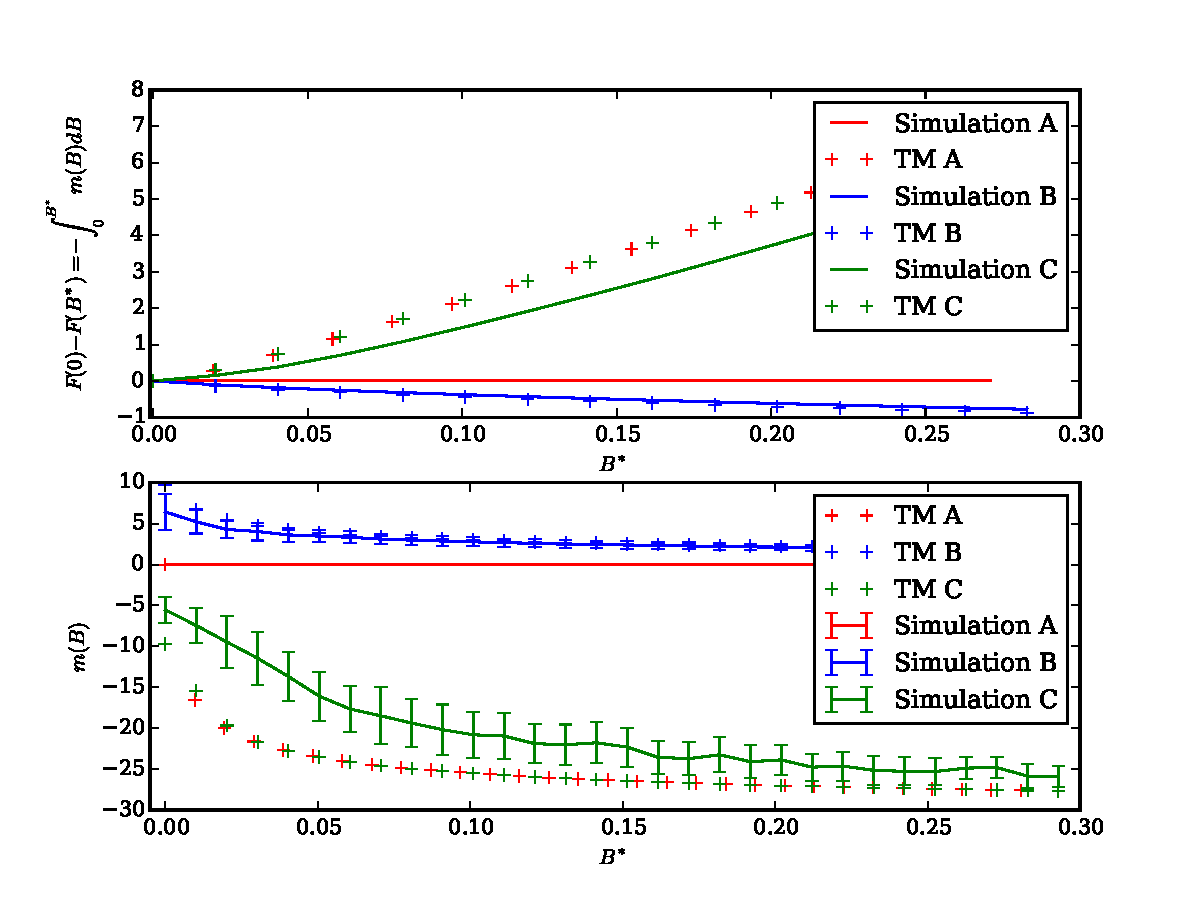
\includegraphics[width=13cm]{ModKaw.pdf}
		  \caption{Computation of the free energy (above) and the magnetisation (below) for the three models in a Kawasaki dynamics (constrained dynamics) through simulations (with error bars) and exact transfer matrix diagonalization. The error in magnetization of Model A is exactly equal to 0, by construction.}
		  \label{compKaw}  
		\end{figure}

  \section{Discretization of the system with respect to continuous models}
    \subsection{Correlation length and temperature}
\end{comment}